%\documentclass[3p,twocolumn]{article}
\documentclass[12pt]{article}

\usepackage{graphicx}
\usepackage{color}
\usepackage{url}
\usepackage{ifpdf}
\usepackage{hyperref}
\usepackage{xspace}
%\usepackage[draft]{pdfdraftcopy}

\setlength\parskip{-0.015em}
\setlength\parsep{-0.15em}

\newenvironment{shortlist}{
	\vspace*{-0.85em}
  \begin{itemize}
 \setlength{\itemsep}{-0.3em}
}{
  \end{itemize}
	\vspace*{-0.6em}
}

\usepackage{fullpage}
%\usepackage[top=tlength, bottom=blength, left=llength, right=rlength]{geometry} %http://en.wikibooks.org/wiki/LaTeX/Page_Layout
%\usepackage[margin=1in, paperwidth=5.5in, paperheight=8.5in]{geometry}

\usepackage{fancyhdr}
\setlength{\headheight}{16.0pt}
\pagestyle{fancy}
\headheight = 0pt
\headsep    = 25pt
\fancyhf{}
%\fancyhead[OC]{\bf {\it \footnotesize{Jha et al: A Case for SAGA as an Access Layer for DCI}}}

\newif\ifdraft
\drafttrue
\ifdraft
 \newcommand{\amnote}[1]{  {\textcolor{magenta} {***AM: #1}}}
 \newcommand{\jhanote}[1]{ {\textcolor{red}     {***SJ: #1}}}
 \newcommand{\olenote}[1]{ {\textcolor{blue}    {***OW: #1}}}
\else
 \newcommand{\amnote}[1]{}
 \newcommand{\jhanote}[1]{}
 \newcommand{\olenote}[1]{}
\fi

\newcommand{\dn}{\vspace*{0.33em}}
\newcommand{\dnn}{\vspace*{0.66em}}
\newcommand{\dnnn}{\vspace*{1em}}
\newcommand{\uppp}{\vspace*{-1em}}
\newcommand{\upp}{\vspace*{-0.66em}}
\newcommand{\up}{\vspace*{-0.33em}}
\newcommand{\shift}{\hspace*{1.00em}}

\newcommand{\T}[1]{\texttt{#1}}
\newcommand{\I}[1]{\textit{#1}}
\newcommand{\B}[1]{\textbf{#1}}
\newcommand{\BI}[1]{\B{\I{#1}}}
\newcommand{\F}[1]{\B{[FIXME: #1]}}
\newcommand{\TODO}[1]{\textcolor{red}{\B{TODO: #1}}}

\begin{document}

\title{Towards a Scalable Architecture for Deep Sequencing Analytics}

\author{Joohyun Kim$^{1}$, Sharath Maddineni$^{1}$, Shantenu Jha$^{*1,2}$, \\
  \small{\emph{$^{1}$Center for Computation \& Technology, Louisiana State University, USA}}\\
  \small{\emph{$^{2}$Department of Computer Science, Louisiana State University, USA}}\\
  \small{\emph{$^{*}$Contact Author \texttt{sjha@cct.lsu.edu}}}
  }


\maketitle

\section*{Abstract}

We investigate the use of distributed computing environments, a
production HPC grid and a cloud environment for the genome-wide
mapping with BFAST.  The main goal of this work is to understand the
characteristics of these two distributed computing environments and
compare and contrast their strengths and suitability to support the
computational requirements of deep sequencing.
% regarding computational requirements of the target bioinformatics
% application whose 

We investigate two model genomes -- human genome and a microbe,
Burkerholderia Glumae, that might represent a eukaryote and a
prokaryote system.  The computational complexity of execution of bioinformatics calculation, mapping with BFAST, 
depends upon the size of a reference genome, the data size of short
reads from high-throughput technologies of the Next Generation
Sequencing platforms, and their biological genome contexts such as distinctive differences between prokaryotes vs eukaryotes.

The two distributed environments, the Louisiana Optical Network
Initiative (LONI) grid and a Cloud system from the FutureGrid, were
used primarily focusing on different and unique challenges in HPC and
Cloud computing conditions.

The time to completion are analyzed by comparing advantages as well as
limitations of each distributed computing infrastructure in
conjunction with distinctively different two different genome systems.
With our results, we discuss the importance of an effective runtime
environment that facilitates a rapid development of
cyberinfrastructure of distributed computing resources and supports
optimized execution patterns for a target scientific application, in
particular, of the data-intensive genome-wide analysis.


\section{Introduction}

% \bibliographystyle{plain}
% \bibliography{egi-white-paper}
High-throughput sequencing techniques provided by Next Generation Sequencing (NGS) platforms have changed biological
sciences and biomedical research dramatically with their comprehensive genome-wide
information as well as a considerably affordable cost compared to previous sequencing techniques based on Sanger sequencing\cite{metzker2010,mardis2008-tig,mardis2008-arghg,gilad2009,mortazavi2008,sorek2010}.  
Owing to the advanced deep sequencing protocols such as ChIP-seq and RNA-seq, high-throughput sequencing techniques becomes essential methodologies in studies   of cell development and differentiation\cite{wang2009-natrevgen,pepke2009,gilad2009,mortazavi2008,sorek2010}.   Resulting influx of biological information about the genome-wide organization and the interaction map that reveal underlying mechanisms of gene expression and regulation in a living cell would lead to major discoveries of effective remedies for various diseases such as cancer, infectious diseases, and dysfunctional diseases caused genetically or by aging\cite{amaral2008,encode2007,baek2008,costa2009,}.    

While high-throughput techniques enjoy extremely high coverage of target genome regions, as referred often with the term, "deep sequencing", the current technologies adopted by NGS platforms such as Illumina GA II and Applied Biosystems SOLiD are limited to generate only short sequence reads generally less than 100 hundred nucleotides in a real setting at the time of this writing.  Consequently, these high volume short reads challenge immediately mapping process on to a reference genome or de novo assembly that are required as the first step for any genome-wide studies\cite{alex2009,trapnell2009,scheibye-alsing2009,pop2002,hernandez2008,farrer2008}.      

The need of computational methods for resolving new challenges and requirements of processing and analyzing
genome sequencing data, therefore, is regarded indispensable for accurate and reliable analysis against high-throughput sequencing data and following genome-wide analyses.  As a result, remarkable advances have been witnessed in recent years and many bioinformatics tools are currently available to the scientific community.  Most of such progresses are associated with development of effective algorithms as well as computational implementation\cite{trapnell2009,bfast2009}.  One important caveat is that as advances of genome sequencing technologies need further innovation such as a single molecule sequencing technology and ever-growing genome data would lead to find novel biological implication, any computational algorithms or implementations with a bioinformatic tool are subject to adopt such progresses or will become less useful if the changes or the current implementation do not reflect new conditions. 

Whereas such advances results in availability of many software tools to the computational biology community. the development of
infrastructure and required software is relatively less recognized for its significance.  This is partly because, in addition to requirement of an understanding of applications of interest in terms of the capability of parallel execution in heterogeneous computing environment, the complexity of biological contexts associated with characteristics of a target genome(s), the volume of relevant genomics data, and importantly, difficulties of utilization of heterogeneous distributed computing resources constitute challenges for introducing an appropriate scalable architecture for the infrastructure.

In this work, as a use case, we primarily focus on the mapping process of short reads from NGS platforms against a reference genome.  The mapping is carried out with BFAST which was chosen specifically for its capability to support parallel and multi-threading supports.  Our investigation with this bioinformatic program would represent a general situation for a bioinformatics tool employed for genome-wide analysis infrastructure.

\jhanote{we want to present a strawman of an architecture based upon
  requirements and a reference implementation of the architecture} In
this work, we present our work on the infrastructure development for
the use of High Performance Computing (HPC) grids and Cloud
environment for genome-wide analysis.

Our strategy is, first to understand characteristics of biological information in conjunction with the capability of the target scientific application, and then, to analyze computational complexity for carrying out mapping process with two exemplary genomes, human genome and a microbial genome, Bukerholderia Glumae.  Base on the results with this analysis, we present the use of our runtime environment, Distributed Adaptive Runtime Environment (DARE), which is built upon SAGA/BigJob abstraction and provides an efficient framework for building biological information infrastructure supporting a wide range of execution patterns while recognizing the potential scalability of deployable computing resources.  Our development with a federated HPC grid, Louisiana Optical Network Initiative (LONI) and a Cloud environment in the FutureGrid is described largely focusing on the comparative analysis on execution of mapping process in each environment. 


%First, we note that in general, genome-wide mapping procedure is an good example of data-intensive scientific applications and can be efficiently carried out with parallel or concurrent executions if there exist ways of data fragmentation with intact biological information.  For example, a reference genome is likely to be composed of many chromosomes or plasmids, and thus mapping on each chromosomes and plasmids can be executed separately.  The challenge, however, is that the way of data fragmentation, and thus system configuration for required parallel/concurrent runs should be considered the characteristics of system environment. Those characteristics differ distinctively between a HPC grid and a Cloud and also vary with a specific target system in each class.  


\section{Mapping with BFAST Tool with Two Genome Datasets : Scientific and Computing Challenges}
\subsection{BFAST : Application}

Our target genome analysis tool is a mapping tool, BFAST\cite{bfast2009,bfast2009b}, which represents a class of tools that comprises diverse genome-wide analysis applications but shares similar computational features.  Such features include i) a requirement of input files containing sequence information of a reference genome or short reads from NGS platforms ii) a production of output files that is generally written with a format that is successively injected to another tool as input.  These aspects, along with a huge variation in the data volume in input, output, or temporary files, often require that the tool should support parallel or multi-threading executions, which is also true with BFAST\cite{bfast2009}.  

As summarized in Fig.~\ref{fig:workflow-bfast} and Table~\ref{table:bfast-summary}, BFAST carries out a pipeline that comprises six different steps (using a different command), and compute extensive steps could be executed in parallel or multi-threading support options.  In brief, BFAST requires a reference genome sequence and NGS platform generated short reads initially and prepare input files with pre-defined formats.  Then, the program carries out indexing of the reference genome, finding Candidate Alignment Locations (CALs), local alignment of CALs, and post-processing of alignment results, which taken together produces the mapping of billions of short reads onto the target reference genome.  Among the steps, three steps (index, match, loalalign) demands most of computing times and computing requirements with the size of a reference genome as well as volumes of short reads.  If computing requirement is high, as stated, BFAST can be executed using parallel or concurrent options by splitting the input data, short reads and a reference genome and run many independent tasks with a part of datasets.  For example, short reads files can be prepared with multiple files and short reads in each file are mapped independently against a reference genome.  Meanwhile, where as a reference genome is also split into many files by considering the existence of multiple contigs in an entire genome, for example, multiple chromosomes and plasmids, in the case of one large sequence, all information about indexing should be treated as a whole for "match" step. 

BFAST also supports multi-threading and the low memory option for "match" step. Once a reference genome sequence is given and not able to be split into further, creating indexes of the reference genome with multiple index files are possible resulting the number of the index files, $N_i$ equal to $n_m \times 4^d$ where d is the parameter for the low memory consumption and $4^d$ files are generated by splitting an index file.  $n_m$ is the number of masks for indexing and usually fixed as 10 for our work.  Whereas this low memory option allows to consume less memory by splitting the information about index into many files and processing sequentially, the number of index files increases.  Another important option provided by BFAST is multi-threading.  If there is multi-core in a node, the option can specify the number of cores for multi-threading.    

\begin{figure}
 \centering
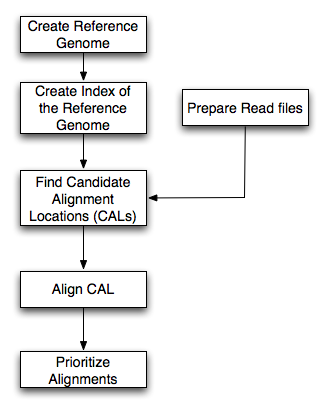
\includegraphics[scale=0.45]{figures/workflow.png} 

\caption{\small Overall workflow for a mapping procedure using BFAST.  In this work, we focus on the step for finding Candidate Alignment Locations (CALs).  }
  \label{fig:workflow-bfast} 
 \end{figure}


\begin{table}
\begin{tabular}{|c|c|c|c|} 
  \hline 
 BFAST command & Description & Computing  Requirement  \\ 
  &  &     for Parallel Strategy \\\hline
bfast fasta2brg & creation of a ref. genome  &    multiple independent contigs \\
&  preparation of short reads files &     multiple sequence reads files \\
  bfast index & creation of reference genome indexes& multi-threading, split index file creation\\
 bfast match & finding candidate alignment locations  &  multi-threading, parallel execution \\
 bfast localalign & alignment of each CAL  &   parallel execution \\
bfast postprocess & prioritization of alignments  &  parallel execution \\ \hline


\hline
\end{tabular} \caption{Description of BFAST commands and computational requirements}
 \label{table:bfast-summary} 
\end{table}

%Note that the number of required
%concurrent tasks, $N$, 


\subsection{BFAST: Characteristics}

\begin{figure}
 \centering
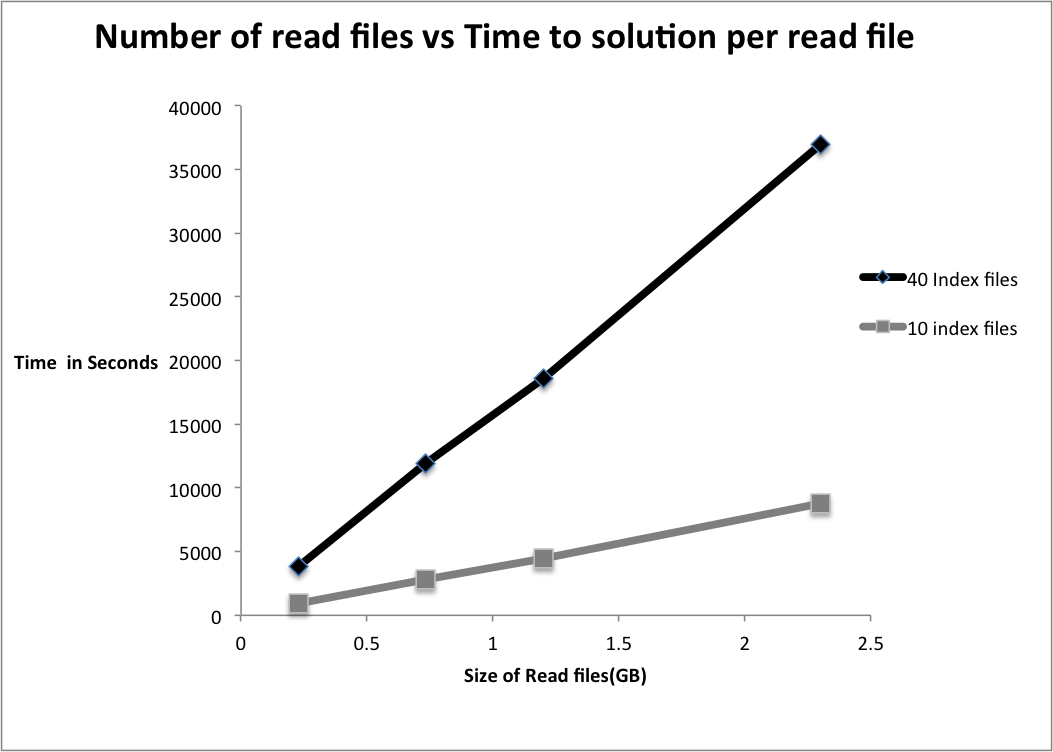
\includegraphics[scale=0.43]{figures/readvstime.png}
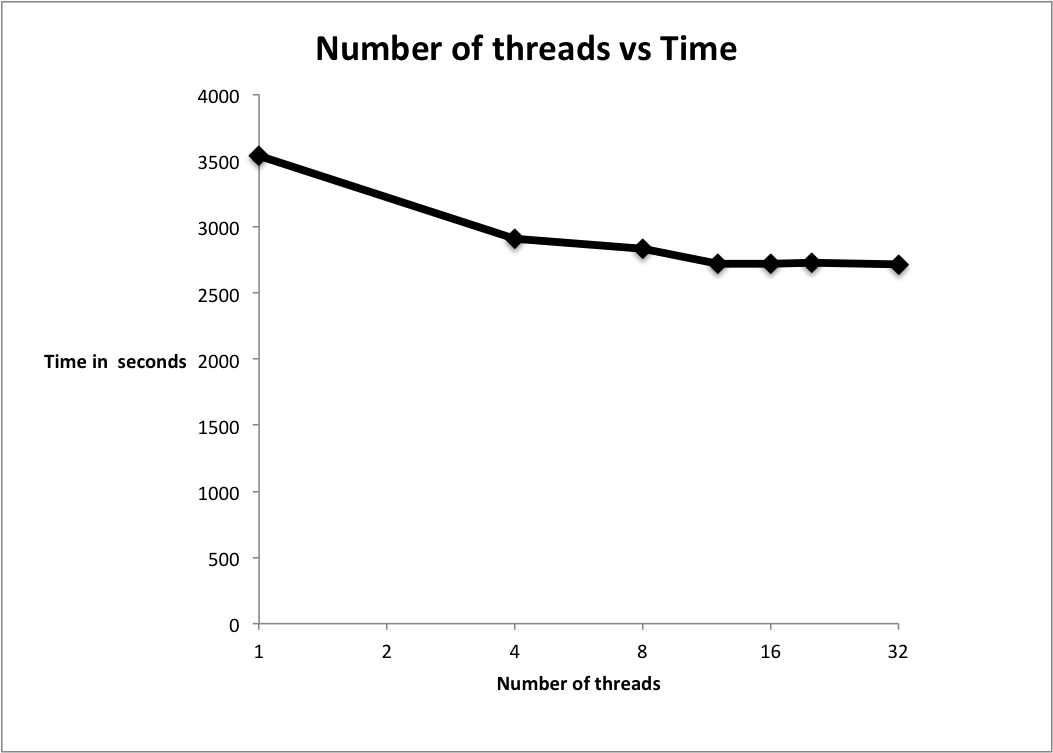
\includegraphics[scale=0.44]{figures/threadsvstime.png} 

\caption{\small Parallel execution support in BFAST.  "match" step is measured by changing the size of short reads file and low memory option (left) and multi-threading support (right).  Human genome (hg18) chromosome 21 is used as the reference genome}
  \label{fig:parallel-execution} 
 \end{figure}


The time-to-solution for "match" step depends upon several parameters that determine the configuration for parallel tasks and multi-threading support.  Computational resource specification such as the size of memory, accessible volume of disk space, the number of cores in a node, and the total number of cores available are the important information for optimal condition for such parameters.  An understanding of such aspects was attempted by characterizing computing characteristics of the "bfast match" step.  The results from our investigation are presented  in Fig.~\ref{fig:parallel-execution}. First, performance gains with multi-threading are marginal showing only 30 \% speed up when reaches the limit with all of the number of free cores being used.  
Secondly, the multiple reads file option is useful as a strategy for scaling out, i.e. with more cores operating correspondingly a smaller reads file.  Thirdly, the low memory option that creates more index files require longer calculation time as the comparison between 40 index files $(d = 1)$ vs. 10 index files ($ d = 0 $) and $n_m = 10$.   





\begin{table}
\begin{tabular}{|c|cc|} 
  \hline 
  Genome Species & Human  & Burkerholderia Glumae  \\ \hline
  Type of Genome Analysis &  Exome  & Whole Genome Resequencing \\
  Sequencing Platform & ABI SOLiD  &  Illumina GA2 \\
  Num. of nucleotides in a Reference Genome (in bp) &  3 G & 7.3 M \\
  Size of Sequencing Data (.fastq) (in Byte) & 8.7G & 5.4 G \\

\hline
\end{tabular} \caption{Specification of target genomes and sequencing data from Next Generation Sequencing (NGS) platforms.}
 \label{table:two-genomes} 
\end{table}

\subsection{Computational Requirements}

Computational requirements for carrying out the "bfast match" step are closely connected biological contents such as a target reference genome and type of short reads, parallel/multi-threading configuration, and available computing architectures.  

To understand computational requirements arising from different biological aims, we examined the two genome datasets and compared the results. Two genomes represents two extremes, an eucaryote system, human, and a microbe, Burkerholderia Glumae\cite{kim2011} that differ in the size and the genome structure of reference genomes, types of sequencing protocols for generating short reads and consequently different mapping rates, which is summarized in Table~\ref{table:two-genomes}, 

Computational requirements are also associated with how to configure parallel/multi-threading execution patterns, and the results shown in Fig.~\ref{fig:parallel-execution} could be utilized for the prediction of such requirements for a desirable scenario, for example, the shortest time to solution case. 

Importantly, the implementation of multiple tasks needs to pay attention on the data volume since in some cases, a large volume of data comprising a reference genome sequence, indexes of the reference genome, short reads, and temporary files prohibits to utilize a computing resource with the limited disk space or the memory.  For example, in Table~\ref{}, we illustrate the minimum disk space for carrying out "bfast match" with typical cases of parallel scenarios.




\jhanote{Joohyun: Please organize each description addressing each of
  the following points: (i) Brief outline of the scientific problem,
  (ii) What are the challenges, (iii) estimates of volumes of data
  involved, distributed or not?, number of tasks, are they coupled or
  uncoupled -- what is the level of coupling between tasks?}


 \begin{table}
 \begin{tabular}{|c|cc|} 
 \hline 
Distributed Environment &  HPC Grid &  Cloud \\ \hline
System  &  Louisiana Optical Network Initiative & FutureGrid \\
Name &  QB/Eric   &  INDIA/SIERRA \\
 \hline
 \end{tabular}
\caption{Specification of two distributed environments}
\label{table:two-systems} 
\end{table}
 
 
\section{Existing Solutions: Limitations and Challenges}

\jhanote{Here we need to define what solutions are currently employed, what works well
  what doesn't}

\begin{itemize}
\item CloudBurst\cite{cloudburst}
\item CouldBlast\cite{cloudblast}
\item SNP finding with Cloud\cite{langmead2009}
\end{itemize}


\section{Distributed, Scalable Architectures}

The DARE framework, comprising an open source Web application, Pylons
and the runtime environment for distributed scientific applications,
was employed for this work.  The framework enables us to develop a
lightweight, extensible, full-fledged science gateway effectively in
which the runtime environment built upon SAGA and BigJob abstraction
manages efficiently distributed computing-driven execution patterns of
target scientific applications.

There are two steps for the BFAST implementation. First step is to prepare read files in the 
fastq format and in the second step we run matching using BFAST with the prepared read files.
 We can generate as many number of read files as we want in the first step in the first step
 but the second step could be scaled with more number of tasks. Because the number tasks 
 in the second step is determined by the number read files we prepare in the first step. We 
 can generate as many number of read files as we want in the first step. We can use as many resources/machines 
 in this step as the tasks are not coupled to each other but the problem is we need the transfer the appropriate read file
in to the respective resource.

37 tasks for the second step was chosen arbitrarily to show the scaling  and to find the performance 
difference with concurrent tasks in the second step. So 37 read files should be prepared in the
 first step by setting the parameters accordingly.

We use SAGA-BigJob to implement the above two steps on grids and clouds and 
the architecture remains BigJob remains same for both grids and clouds. All the first 
step jobs and second step jobs are defined as subjobs in the BigJob. At first only 
one job is submitted ie  preparing the read files and the jobs in the second step are not submitted
until the first job is done. Once the Read files are prepared the 37 subjobs are submitted in to 
job queue of the Bigjob. Number of concurrent subjobs that can be processed depending 
on the available cores that are requested in the BigJob.
  
In the Grid implementation first all the data required in the steps was transferred to machine's  work 
directory where we want to start the BigJob. The Bfast was installed in the home directory and the
executables path for job description of subjobs was given accordingly.

In the cloud implementation all the data required was transferred into the walrus because of the data size limitation of the storage space in the
running VM. Multiple VM's can be started at once and the data in the walrus is mounted onto all the running VM
while booting the Virtual Machine. Thus all the VM can have access to data and can process concurrently



\section{Concluding Remarks}
We present our analyses with two genome systems representing a eukaryote and a prokaryote, respectively, using
 a HPC grid and a Cloud environment for an understanding of conditions of a scalable cyberinfrastructure for an effective execution of
 mapping, and consequently genome-wide analyses.   Based on our results, we conclude that an infrastructure to run with a proper configuration for concurrent tasks benefits genome-wide analysis and such a configuration is optimized only when parameters from biological contexts as well as limitations and potentials of distributed computational resources are taken into account together.  For that purpose, our DARE framework provides an efficient solution.  



\bibliographystyle{abbrv}
\bibliography{ecmls11}


\end{document}

